%#!platex master-ohp.tex
\documentclass{slides}
%#!platex master.tex
% Packages used
\usepackage{graphicx}
\usepackage{color}
\usepackage{amsmath}
\usepackage{amssymb}
\usepackage{amsfonts}
\usepackage{amsthm}
\usepackage{amsxtra}
\usepackage{mathrsfs}
\usepackage[all]{xypic}
\usepackage{enumerate}

% \CompileMatrices
% Define theorem environment
\newtheoremstyle{mythmsty}{3pt}{3pt}{\upshape}{}{\upshape\bfseries}{}{\newline}{}
\theoremstyle{mythmsty}
\renewcommand{\proofname}{{\bfseries $B>ZL@(B}}
\newtheorem{The}{$BDjM}(B}[section]
\newtheorem{Def}[The]{$BDj5A(B}
\newtheorem{Lem}[The]{$BJdBj(B}
\newtheorem{Cor}[The]{$B7O(B}
\newtheorem{Conj}[The]{$B2>@b(B}

%make upshape default
\upshape

% Some outlooks
\setlength{\textwidth}{150mm}
% for jbook
\renewcommand{\bibname}{$B;29MJ88%(B}
\setlength{\evensidemargin}{-3mm}
\setlength{\oddsidemargin}{7mm}
% for jreport
%\setlength{\evensidemargin}{5mm}
%\setlength{\oddsidemargin}{5mm}

%Some abbreviations
\def\sla#1{\rlap{\kern .15em /}#1}
\def\bra#1{\langle #1 |}
\def\ket#1{| #1 \rangle}
\def\ten{\textperiodcentered}
\def\der{\partial}
\def\1half{\frac{1}{2}}
\def\ihalf{\frac{i}{2}}
\def\kbar{{\mathchar'26\mkern-9muk}}

\def\vl{\vec{l}}
\def\vk{\vec{k}}
\def\vp{\vec{p}}
\def\ap{{\alpha'}}
\def\ls{{\ell_{\mathrm{s}}}}
\def\Ud{U^\dagger{}}

\def\rht{{\tilde{\rho}}}
\def\Kt{{\tilde{K}}}
\def\Ab{{\bar{A}}}
\def\At{{\tilde{A}}}
\def\Ah{{\hat{A}}}
\def\Dh{{\hat{D}}}
\def\Dt{{\tilde{D}}}
\def\Fh{{\tilde{F}}}
\def\Ft{{\tilde{F}}}
\def\xh{{\hat{x}}}
\def\yh{{\hat{y}}}
\def\zb{{\bar{z}}}
\def\derb{{\bar{\partial}}}
\def\delh{{\hat{\delta}}}
\def\delt{{\tilde{\delta}}}
\def\lamh{{\hat{\lambda}}}
\def\lamt{{\tilde{\lambda}}}
\def\theh{{\hat{\theta}}}
\def\thet{{\tilde{\theta}}}

\def\Cst{\mathrm{C}^*{}}
\def\Cinf{\mathrm{C}^\infty}

\def\crea{a^\dagger{}}
\def\anih{a}
\def\creC{{C^*}}
\def\aniC{{C}}
\def\Sd{{S^*}}
\def\Tb{{T^*}}


\def\zero{\mathbf{0}}
\def\E{\mathrm{e}}

\def\Ad{\mathrm{Ad}}
\def\Aut{\mathrm{Aut}}
\def\Arg{\mathrm{Arg}}
\def\CoD{\mathrm{cod}\,}
\def\Diag{\mathrm{diag}}
\def\Dim{\mathrm{dim}}
\def\Dom{\mathrm{dom}\,}
\def\End{\mathrm{End}}
\def\Ext{\mathrm{\mathbf{Ext}}}
\def\GL{\mathrm{GL}}
\def\Ham{\mathrm{H}}
\def\Hom{\mathrm{Hom}}
\def\Ker{\mathrm{Ker}}
\def\id{\mathrm{id}}
\def\Img{\mathrm{Im}}
\def\Ind{\mathrm{Index}}
\def\n{\mathrm{n}}
\def\Ob{\mathrm{Ob}}
\def\Rank{\mathrm{Rank}}
\def\Tr{\mathrm{Tr}}
\def\Vect{\mathrm{Vect}}


\def\bx{\mathbf{x}}
\def\AlgA{\mathcal{A}}
\def\AlgAk{{\mathcal{A}_\kbar}}
\def\AlgB{\mathcal{B}}
\def\AlgC{\mathcal{C}}
\def\AlgJ{\mathcal{J}}
\def\AlgK{\mathcal{K}}
\def\CatA{\mathscr{A}}
\def\CatB{\mathscr{B}}
\def\CatC{\mathscr{C}}
\def\ModM{\mathcal{M}}
\def\ModN{\mathcal{N}}
\def\ModE{\mathcal{E}}
\def\ModF{\mathcal{F}}
\def\Mat{\mathrm{Mat}}
\def\MatK{\mathbb{K}}
\def\Mtrx{\mathbb{M}}
\def\Minf{{\mathbb{M}_\infty}}
\def\OpO{\mathcal{O}}
\def\Toep{\mathcal{T}}
\def\Spi{\mathcal{S}}

\def\Real{\mathbb{R}}
\def\Cplx{\mathbb{C}}
\def\Rtnl{\mathbb{Q}}
\def\Hil{\mathscr{H}}
\def\Intg{\mathbb{Z}}
\def\Ntrl{\mathbb{N}}
\def\Ord{\mathcal{O}}
\def\Trvn{\mathfrak{n}}
\def\Trvm{\mathfrak{m}}


\def\AntiSymBlock#1{
\begin{matrix}
 0   & #1 \\
 -#1 & 0  \\
\end{matrix}}


\begin{document}

$U(\infty)$$B$NBP>N@-$r2u$7$F$7$^$&!#(B\\
$\Rightarrow U(1)$$B%2!<%8>l$rF3F~$9$k$H(B$U(\infty)$$B$,I|3h!#(B

$\color{blue}x,y$$B$,$b$O$d8r49$7$J$$$N$G!"(B$\color{blue}x,y$$B$G1i;;;R7A<0$G(B
$B=q$$$?%O%_%k%H%K%"%s$O!"(B
\[\color{blue}
  \Ham=2\pi\Tr\left(\1half([\aniC,\creC]+1)^2
		 +[\aniC,\phi][\creC,\phi]
		 +\theta V(\phi)\right)
\]
\[\color{blue}
 \creC\equiv \crea+i\theta^{\1half}A,\quad
  \aniC\equiv \anih-i\theta^{\1half}\Ab\quad\mbox{($B6&JQHyJ,(B)}
\]
$B$3$3$G!"(B$U(\infty)$$B$NBP>N@-$,$"$k$H!"(B{\color{red} Solution generating
technique}$B$r;H$&$3$H$,$G$-$k!#$D$^$j0J2<$N$h$&$JJQ49$r$9$k$H!"(B
\underline{\color{blue} $B?7$7$$2r$r9=@.$G$-$k!#(B}
\[\color{blue}
 C\rightarrow SC\Sd,\quad\phi\rightarrow S\phi\Sd
\]
$B$3$3$G!"(B$S$$B$O(B{\color{red} isometry}$B$D$^$j!"(B\ovalbox{\color{blue}$\Sd
S=1$}$B$rK~$?$9!#(B\\
$BNc$($P(B$S$$B$,(Bshift operator \ovalbox{\color{blue}$S\equiv
\sum\limits_{k=0}^\infty \ket{k+1}\bra{k}$}$B$N;~(B
\[\color{blue}
 \left\{\begin{array}{l}
  \phi=\phi_*\\
  A=0\\
  E=0
 \end{array}\right.\mbox{\shortstack[c]{$S^n$\\ $\Rightarrow$}}
 \left\{\begin{array}{l}
  \phi=\phi_*(1-\sum\limits^{n-1}_{k=0}\ket{k}\bra{k}) \\
  \aniC=S^n\crea\Sd^n,\,\creC=S^n\anih\Sd^n \\
  E=2\pi n\left(\frac{1}{2\theta}+\theta V(0)\right)
 \end{array}\right.
\]

\newpage
%%%%%%%%%%%%%%%%%%%%%%%%%%%%%%%%%%%%%%%%%%%%%%%%%%%%%%%%%%%%%%%%%%%%%%%%

\begin{center}
 $B%?%-%*%s>l$N%]%F%s%7%c%k(B
 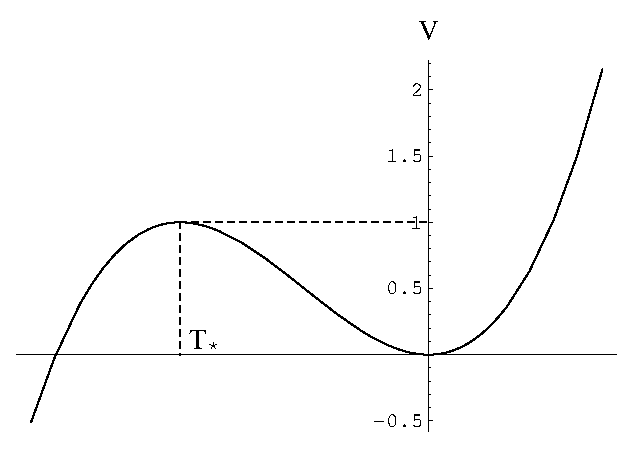
\includegraphics{tachyon-potential.eps}
\end{center}\vspace{-1cm}
Sen$B$N2>@b$K$h$k$H!"IT0BDj$J%?%-%*%s$N$"$k??6u$H%?%-%*%s$NL5$$??6u$H$N%?(B
$B%-%*%s%]%F%s%7%c%k$N:9$O(Bbrane$B$N%F%s%7%g%s$K0lCW$9$k!#(B\\
$\Rightarrow$\parbox{14cm}{$B%?%-%*%s>l$G(B\NCS $B$r9=@.$9$k$H(B,\\
\underline{\color{blue}$B$=$N%F%s%7%g%s$O(BD-brane$B$H0lCW$9$k!#(B}
$B2?8N$J$i$P!"(B2$B<!85$NJ}8~$r(B$\color{blue}$}


$B$5$i$K!"(B\NCS $B2r$N$^$o$j$N%2!<%8>l$N(Bfluctuation$B$r9M$($k$H!"(B\NCS $B$H%2!<%8(B
$B>l$N%+%C%W%j%s%0$N;EJ}$O(B\underline{\color{blue} D-brane$B$N$=$l$H0lCW$9$k!#(B}

$B0J>e$N;v<B$+$i<!$N$3$H$,8@$($=$&!#(B\\
\ovalbox{\parbox{16cm}{\color{blue} \NCS $B$O<B$O(BD-brane$B$rI=(B
$B$o$7$F$$$k!#(B}}

%%%%%%%%%%%%%%%%%%%%%%%%%%%%%%%%%%%%%%%%%%%%%%%%%%%%%%%%%%%%%%%%%%%%%%%

\typeout{=== Region from (point) to (mark) ===}

\end{document}
